\documentclass[10pt,aspectratio=169]{beamer}

\usetheme{metropolis}
\usepackage{appendixnumberbeamer}
\usepackage{booktabs}
\usepackage{siunitx}
\usepackage{xcolor}
\usepackage{tikz}
\usetikzlibrary{positioning, arrows.meta, shapes.geometric, fit, backgrounds, calc}
\usepackage{graphicx}
\graphicspath{{../results/}}

\definecolor{plotblue}{HTML}{1F4E79}
\definecolor{plotred}{HTML}{B85450}
\definecolor{plotgreen}{HTML}{355E3B}
\definecolor{plotpurple}{HTML}{6B4C9A}
\definecolor{plotgray}{HTML}{404040}
\definecolor{plotgridgray}{HTML}{E0E0E0}

\setbeamercolor{normal text}{fg=plotgray, bg=white}
\setbeamercolor{alerted text}{fg=plotred}
\setbeamercolor{example text}{fg=plotgreen}
\setbeamercolor{frametitle}{fg=white, bg=plotblue}
\setbeamercolor{title separator}{fg=plotblue}
\setbeamercolor{progress bar}{fg=plotblue, bg=plotblue!20}
\setbeamercolor{progress bar in section page}{fg=plotblue, bg=plotblue!20}
\setbeamercolor{section title}{fg=plotblue}
\setbeamercolor{block title}{bg=plotblue!15, fg=plotblue}
\setbeamercolor{block body}{bg=plotblue!5}
\setbeamercolor{itemize item}{fg=plotblue}
\setbeamercolor{itemize subitem}{fg=plotred}
\setbeamercolor{enumerate item}{fg=plotblue}
\setbeamercolor{structure}{fg=plotblue}

\title{In-Memory Object Storage in a Single Address Space}
\subtitle{}
\author{Taj Jethwani-Keyser}
\institute{Harvard SEAS}
\date{\today}

\begin{document}

\maketitle

\begin{frame}{Outline}
	\tableofcontents
\end{frame}

\section{Motivation}

\begin{frame}{What is an in-memory object store?}
	\begin{itemize}
		\item A shared key$\to$value table holding live application objects.
        \item Multiple clients (threads or processes) read and write
        concurrently.
		\item Latency profile ranging from nanoseconds to milliseconds.
        \item Used as a cache, a feature store, or a coordination layer between
        tightly coupled services.
          \begin{itemize}
              \item Often accessed remotely, but not always (e.g., data
              pipelines, multi-GPU training).
              \item Focus today is on low-latency intra-server IPC.
          \end{itemize}
	\end{itemize}
\end{frame}

\begin{frame}{In-Memory Bottlenecks}
    Can classify (most) overhead into one of two categories:
	\vspace{0.4em}
	\begin{columns}[T, onlytextwidth]
		\begin{column}{0.48\textwidth}
			\begin{block}{IPC overhead}
				\begin{itemize}\setlength\itemsep{2pt}
                    \item Context-switch on every \texttt{get}/\texttt{put}:
                    \begin{itemize}
                        \item Notify database with \texttt{send}/\texttt{recv}
                        \item Schedule database worker thread
                    \end{itemize}
                    \item Copying values from client memory to server memory and
                    back
				\end{itemize}
			\end{block}
		\end{column}
		\begin{column}{0.48\textwidth}
			\begin{block}{Metadata overhead}
				\begin{itemize}\setlength\itemsep{2pt}
                    \item Synchronization on shared state
                    \begin{itemize}
                        \item Concurrent hash tables, skip lists
                        \item Key/value reference counts
                    \end{itemize}
                    \item Memory access isn't free!
                    \begin{itemize}
                        \item Data cache and TLB misses
                    \end{itemize}
				\end{itemize}
			\end{block}
		\end{column}
	\end{columns}
\end{frame}

\begin{frame}{Related Work}
	\begin{itemize}
        \item ``Rearchitecting In-Memory Object Stores for Low Latency'' (VLDB
        '22).
        \item Elegant solution to the IPC problem:
        \begin{itemize}
            \item Metadata (hash table) and data (raw buffers) allocated from
            a shared memory region.
            \item Clients read/write to database directly via specialized client
            library.
        \end{itemize}
        \item Unsurprisingly, benchmarks are far better than competitors like
        Redis and Plasma.\footnote{deprecated Apache Arrow project}
        \item But\dots focus is placed on safety rather than ``low latency'':
        \begin{itemize}
            \item ``To avoid concurrent modification to the object store’s
            state, we use a single spinlock to serialize client operations\dots
            \, Lightning has the best performance when there is only one client
            because multiple clients can result in lock contention.''
            \item Emphasis on fault isolation (formally verified!).
        \end{itemize}
	\end{itemize}
\end{frame}

\begin{frame}{Towards a Single Address Space}
	\begin{itemize}
        \item Suppose that clients never crash.
        \item Give up on the multi-process model:
        \begin{itemize}
            \item Shared memory is often slower (due to TLB pressure) and harder
            to deal with (must use relative offsets instead of raw pointers)
            than local heap memory.
            \item Ideally, a client can \texttt{put} an arbitrary pointer (e.g.,
            to a graph or sparse matrix) and it is immediately accessible to
            other clients, like in multi-threaded applications.
            \item Lose process isolation, but this is (partially) fixable.
        \end{itemize}
        \item Use faster, harder-to-verify data structures like concurrent hash
        tables.
        \item But maybe it's impractical to refactor your codebase to use
        threads!
	\end{itemize}
	\vspace{1em}
	These motivate a design where \emph{client binaries are loaded into a single
    process at runtime}.
\end{frame}

\section{Approach}

\begin{frame}{System API}
    \begin{itemize}
        \item Clients \texttt{include} a header with database operations,
        resolved at runtime to host code:
        \begin{itemize}
            \item \texttt{put(key, value*, dtor):} insert pointer to value and
            register destructor callback.
            \item \texttt{get(key) -> handle:} retrieve ref-counted pointer to
            value.
            \item \texttt{close(handle):} decrement ref-count, call
            \texttt{dtor} and free when it reaches zero.
        \end{itemize}
        \item Also some convenience functions, like a C++-only RAII helper for
        handles.
        \item Reference counts make the API flexible but are a real bottleneck
        at scale.
    \end{itemize}
\end{frame}

\begin{frame}{System Architecture}
    \centering
    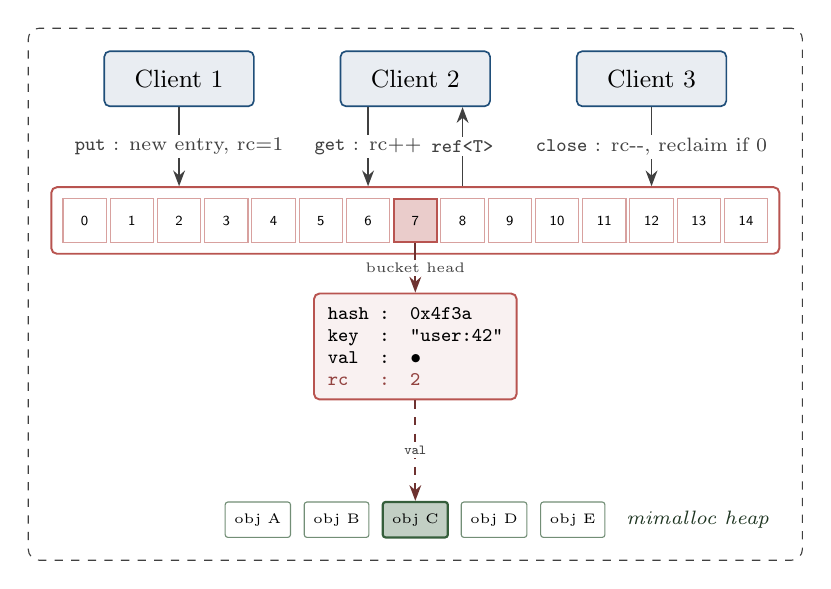
\begin{tikzpicture}[
        font=\small,
        client/.style={rectangle, rounded corners=2pt, draw=plotblue,
                line width=0.6pt, fill=plotblue!10,
                minimum width=1.9cm, minimum height=0.7cm, align=center},
        bucket/.style={rectangle, draw=plotred!55, line width=0.4pt,
                fill=white, minimum width=0.55cm, minimum height=0.55cm,
                font=\tiny\sffamily, inner sep=0pt},
        bucketHL/.style={bucket, draw=plotred, fill=plotred!30,
                line width=0.8pt},
        entry/.style={rectangle, rounded corners=2pt, draw=plotred,
                line width=0.7pt, fill=plotred!8,
                align=left, font=\scriptsize\ttfamily, inner sep=5pt},
        obj/.style={rectangle, rounded corners=1pt, draw=plotgreen!70,
                line width=0.4pt, fill=white,
                minimum width=0.7cm, minimum height=0.45cm, font=\tiny},
        objHL/.style={obj, draw=plotgreen, fill=plotgreen!30, line width=0.8pt},
        arr/.style={-{Stealth[length=2mm]}, plotgray, line width=0.6pt},
        arrlbl/.style={font=\scriptsize, fill=white, inner sep=1.2pt,
                text=plotgray},
        process/.style={rectangle, rounded corners=4pt, draw=plotgray,
                dashed, line width=0.4pt, inner sep=8pt},
    ]

    \node[client] (c1) at (-3.0, 3.4) {Client 1};
    \node[client] (c2) at ( 0.0, 3.4) {Client 2};
    \node[client] (c3) at ( 3.0, 3.4) {Client 3};

    \foreach \i in {0,...,14} {
        \pgfmathsetmacro{\xpos}{-4.2 + 0.6 * \i}
        \pgfmathtruncatemacro{\bidx}{\i}
        \node[bucket] (b\bidx) at (\xpos, 1.6) {\bidx};
    }
    \node[bucketHL] (bH) at (0, 1.6) {7};

    \begin{pgfonlayer}{background}
        \node[draw=plotred, line width=0.7pt, rounded corners=2pt,
              inner sep=4pt, fit=(b0)(b14)] (hashTable) {};
    \end{pgfonlayer}

    \node[entry] (entry) at (0, 0.0) {%
        hash : \texttt{0x4f3a} \\
        key \ : "user:42" \\
        val \ : \(\bullet\)  \\
        \textcolor{plotred!80!black}{\textbf{rc \ \ : 2}}};

    \draw[arr, plotred!60!black] (bH.south) -- (entry.north)
        node[arrlbl, pos=0.5, font=\tiny] {bucket head};

    \node[obj] (oA) at (-2.0, -2.2) {obj A};
    \node[obj] (oB) at (-1.0, -2.2) {obj B};
    \node[objHL] (oC) at ( 0.0, -2.2) {obj C};
    \node[obj] (oD) at ( 1.0, -2.2) {obj D};
    \node[obj] (oE) at ( 2.0, -2.2) {obj E};

    \node[font=\scriptsize\itshape, plotgreen!55!black, anchor=west]
        (heapLabel) at ([xshift=4pt]oE.east)
        {mimalloc heap};

    \draw[arr, dashed, plotred!60!black]
        (entry.south) -- (oC.north)
        node[arrlbl, pos=0.5, font=\tiny] {\texttt{val}};

    \draw[arr] (c1.south) -- (c1.south |- hashTable.north)
        node[arrlbl, midway] {\texttt{put} : new entry, rc=1};

    \draw[arr] ([xshift=-0.6cm]c2.south) --
        ([xshift=-0.6cm]c2.south |- hashTable.north)
        node[arrlbl, midway] {\texttt{get} : rc++};
    \draw[arr] ([xshift=0.6cm]c2.south |- hashTable.north) --
        ([xshift=0.6cm]c2.south)
        node[arrlbl, midway] {\texttt{ref<T>}};

    \draw[arr] (c3.south) -- (c3.south |- hashTable.north)
        node[arrlbl, midway] {\texttt{close} : rc-{}-, reclaim if 0};

    \begin{pgfonlayer}{background}
        \node[process,
            fit=(c1)(c3)(hashTable)(entry)(oA)(heapLabel)]
            (proc) {};
    \end{pgfonlayer}
    \end{tikzpicture}
\end{frame}

\begin{frame}{Concurrent Hash Tables}
    \begin{itemize}
        \item For the database backend, prioritize throughput and tail latency
        at high concurrency.
        \item Initially tried \texttt{boost::concurrent\_flat\_map}:
        \begin{itemize}
            \item Flat open-addressing scheme that uses SIMD for hash lookups.
            \item Striped read-write locks and stop-the-world resizes.
        \end{itemize}
        \item Optimization: store atomic pointers and use CAS for writes.
        \begin{itemize}
            \item Allows updates while holding a read lock instead of a write
            lock.
            \item But requires more advanced reclamation strategies (see next
            slide).
        \end{itemize}
        \item Even better: fully lock-free hash table with chained buckets and
        cooperative resizes.
    \end{itemize}
\end{frame}

\begin{frame}{Safe Memory Reclamation}
    \begin{itemize}
        \item Approaches \#2 and \#3 require synchronization to ensure that a
        value is not freed between retrieving the pointer and incrementing the
        ref-count.
        \item Traditional solution is \emph{epoch-based reclamation}.
        \begin{itemize}
            \item Threads announce a current ``epoch''; values deleted in epoch
            $t$ are not freed until all threads reach epoch $t + 1$.
            \item Single memory barrier per read, but time-to-free is unbounded.
        \end{itemize}
        \item Alternative solution: \emph{hazard pointers}.
        \begin{itemize}
            \item Threads announce the specific pointers they are reading (i.e.,
            the current hash table and value); when freeing a batch of values,
            must check other threads' hazard lists first.
            \item Much heavier and harder to implement, but stalled threads
            block at most two frees.
        \end{itemize}
    \end{itemize}
\end{frame}

\section{Benchmarks}

\begin{frame}{Experimental Setup}
	\begin{itemize}
		\item Workload: Zipfian (\(\theta=0.99\)) over 4M keys, 50\% read/write,
        16 threads.
        \begin{itemize}
            \item Sweep each of these parameters, fix the others.
            \item Workers pinned to a specific core (except TLB benchmark!).
            \item Only microbenchmarks for now; will compare with Lightning on
            YCSB.
        \end{itemize}
        \item Measurement: 5\,s timed window, 2\,s warmup, sampled per-op
        \texttt{rdtsc} (1-of-128 ops).
		\item Hardware: AMD EPYC 7452 (32 cores @ 2.35 GHz), 125 GB memory, 128
        MB L3.
	\end{itemize}
\end{frame}

\begin{frame}{Hash Tables: Concurrency}
    \centering
    \begin{columns}[T, onlytextwidth]
        \column{0.32\textwidth}\centering
            
\includegraphics[width=\linewidth]{backends/num_threads/mixed_throughput.png}\\
            {\scriptsize\itshape Throughput vs. threads}
            
\includegraphics[width=\linewidth]{backends/num_threads/fill_resize_throughput}\\
            {\scriptsize\itshape Fill throughput vs. threads}
        \column{0.32\textwidth}\centering
            
\includegraphics[width=\linewidth]{backends/num_threads/mixed_rd_p99.png}\\
            {\scriptsize\itshape Read p99 latency vs. threads}
            
\includegraphics[width=\linewidth]{backends/num_threads/fill_resize_wr_p99.png}\\
            {\scriptsize\itshape Fill p99 latency vs. threads}
        \column{0.32\textwidth}\centering
            
\includegraphics[width=\linewidth]{backends/num_threads/mixed_wr_p99.png}\\
            {\scriptsize\itshape Write p99 latency vs. threads}
            
\includegraphics[width=\linewidth]{backends/num_threads/fill_resize_wr_p999.png}\\
            {\scriptsize\itshape Fill p999 latency vs. threads}
    \end{columns}
\end{frame}

\begin{frame}{Hash Tables: Working Set}
    \centering
    \begin{columns}[T, onlytextwidth]
        \column{0.32\textwidth}\centering
            
\includegraphics[width=\linewidth]{backends/num_keys/mixed_throughput.png}\\
            {\scriptsize\itshape Throughput vs. working set}
            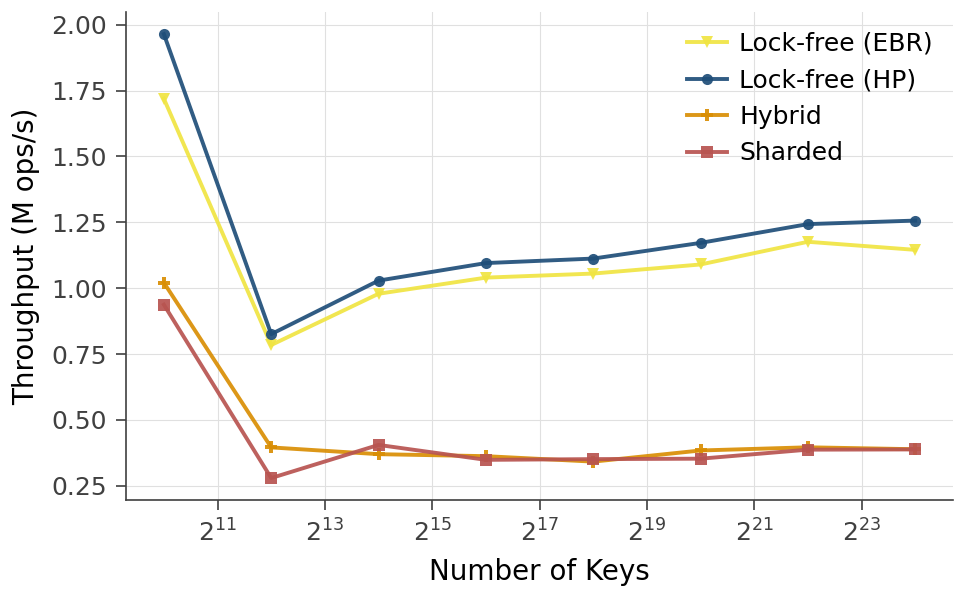
\includegraphics[width=\linewidth]{backends/num_keys/fill_resize_throughput}\\
            {\scriptsize\itshape Fill throughput vs. working set}
        \column{0.32\textwidth}\centering
            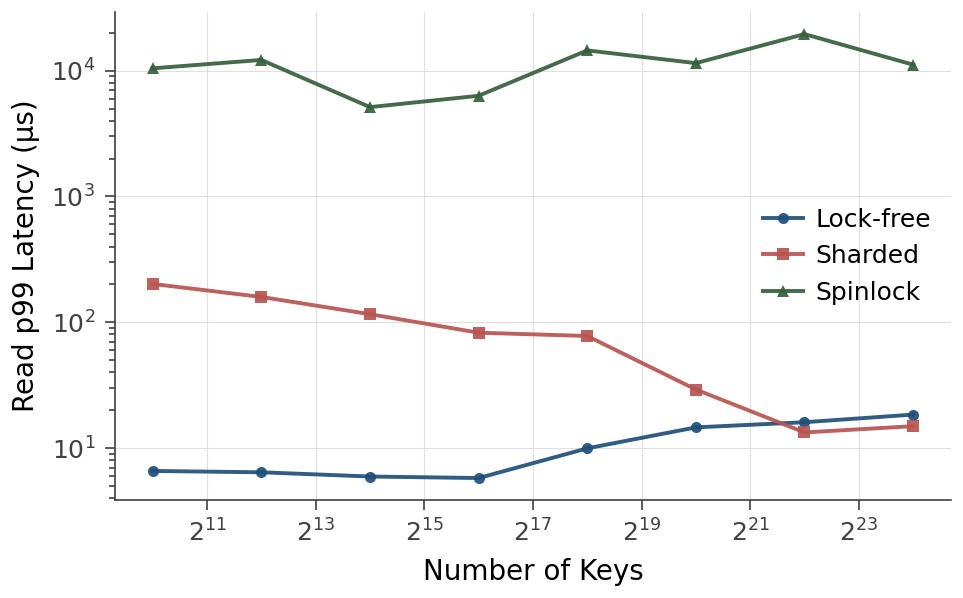
\includegraphics[width=\linewidth]{backends/num_keys/mixed_rd_p99.png}\\
            {\scriptsize\itshape Read p99 latency vs. working set}
            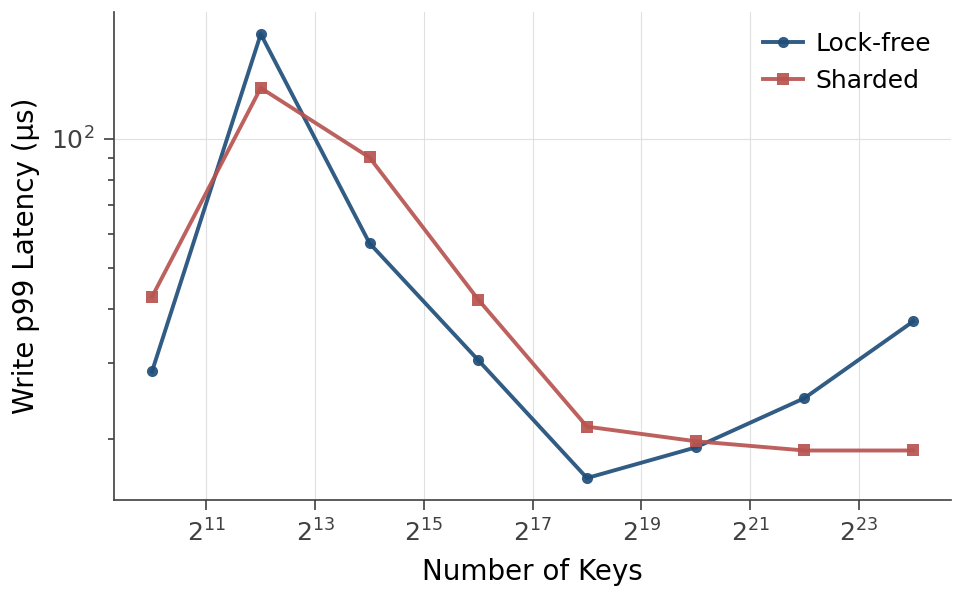
\includegraphics[width=\linewidth]{backends/num_keys/fill_resize_wr_p99.png}\\
            {\scriptsize\itshape Fill p99 latency vs. working set}
        \column{0.32\textwidth}\centering
            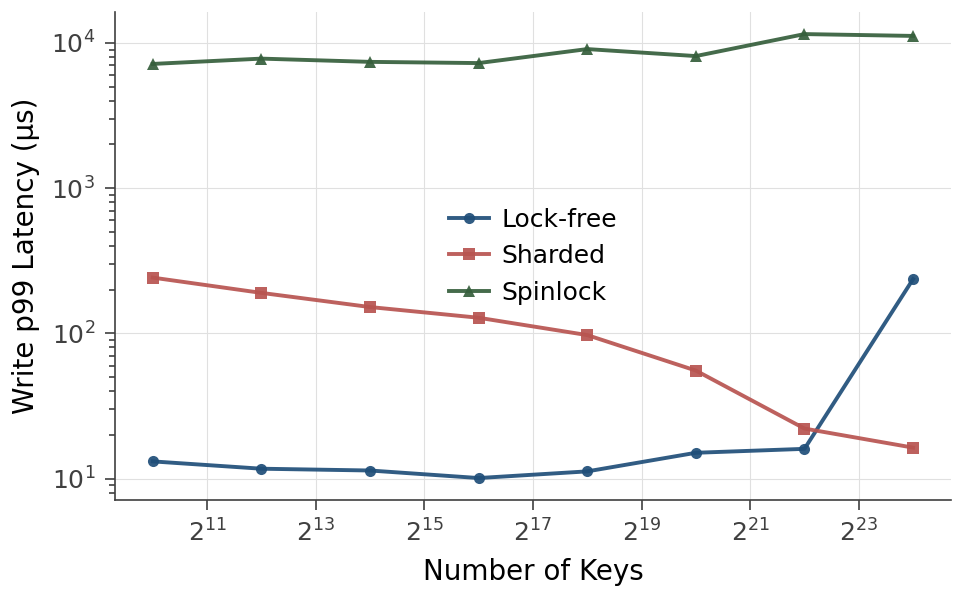
\includegraphics[width=\linewidth]{backends/num_keys/mixed_wr_p99.png}\\
            {\scriptsize\itshape Write p99 latency vs. working set}
            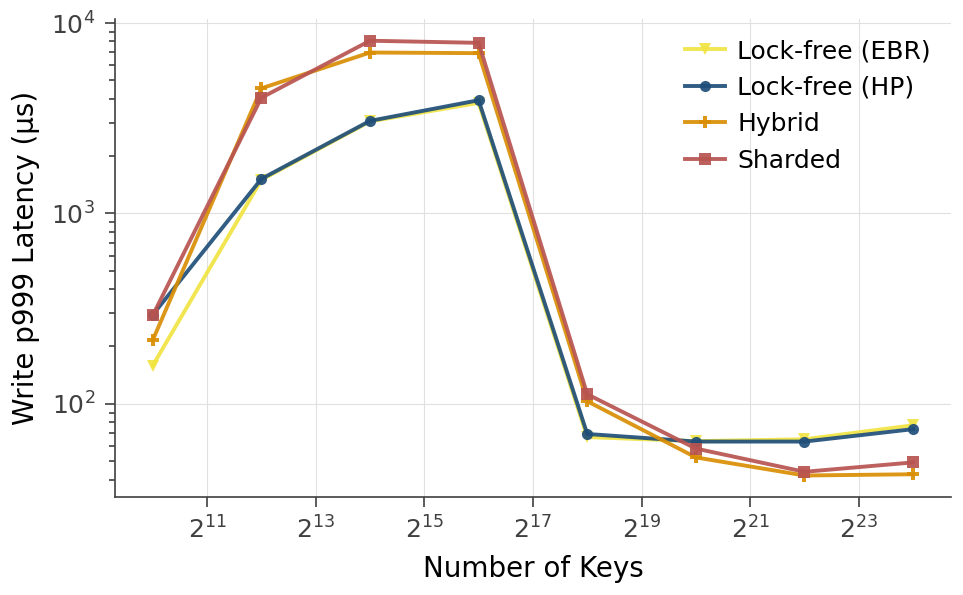
\includegraphics[width=\linewidth]{backends/num_keys/fill_resize_wr_p999.png}\\
            {\scriptsize\itshape Fill p999 latency vs. working set}
    \end{columns}
\end{frame}

\begin{frame}{Hash Tables: Zipfian $\theta$}
    \centering
    \begin{columns}[T, onlytextwidth]
        \column{0.32\textwidth}\centering
            
\includegraphics[width=\linewidth]{backends/zipf_theta/mixed_throughput.png}\\
            {\scriptsize\itshape Throughput vs. $\theta$}
            
\includegraphics[width=\linewidth]{backends/zipf_theta/fill_resize_throughput}\\
            {\scriptsize\itshape Fill throughput vs. $\theta$}
        \column{0.32\textwidth}\centering
            
\includegraphics[width=\linewidth]{backends/zipf_theta/mixed_rd_p99.png}\\
            {\scriptsize\itshape Read p99 latency vs. $\theta$}
            
\includegraphics[width=\linewidth]{backends/zipf_theta/fill_resize_wr_p99.png}\\
            {\scriptsize\itshape Fill p99 latency vs. $\theta$}
        \column{0.32\textwidth}\centering
            
\includegraphics[width=\linewidth]{backends/zipf_theta/mixed_wr_p99.png}\\
            {\scriptsize\itshape Write p99 latency vs. $\theta$}
            
\includegraphics[width=\linewidth]{backends/zipf_theta/fill_resize_wr_p999.png}\\
            {\scriptsize\itshape Fill p999 latency vs. $\theta$}
    \end{columns}
\end{frame}

\begin{frame}{Client Library Overhead}
    \centering
    \begin{columns}[T, onlytextwidth]
        \column{0.32\textwidth}\centering
            
\includegraphics[width=\linewidth]{client_overhead/num_threads/mixed_throughput.png}\\
            {\scriptsize\itshape Throughput vs. threads}
        \column{0.32\textwidth}\centering
            
\includegraphics[width=\linewidth]{client_overhead/num_threads/mixed_rd_p99.png}\\
            {\scriptsize\itshape Read p99 latency vs. threads}
        \column{0.32\textwidth}\centering
            
\includegraphics[width=\linewidth]{client_overhead/num_threads/mixed_wr_p99.png}\\
            {\scriptsize\itshape Write p99 latency vs. threads}
    \end{columns}
\end{frame}

\begin{frame}{Shared Memory Overhead}
    \centering
    \begin{columns}[T, onlytextwidth]
        \column{0.46\textwidth}\centering
            
\includegraphics[width=\linewidth]{arch/num_threads/mixed_throughput.png}\\
            {\scriptsize\itshape Throughput + TLB misses vs. threads}
        \column{0.46\textwidth}\centering
            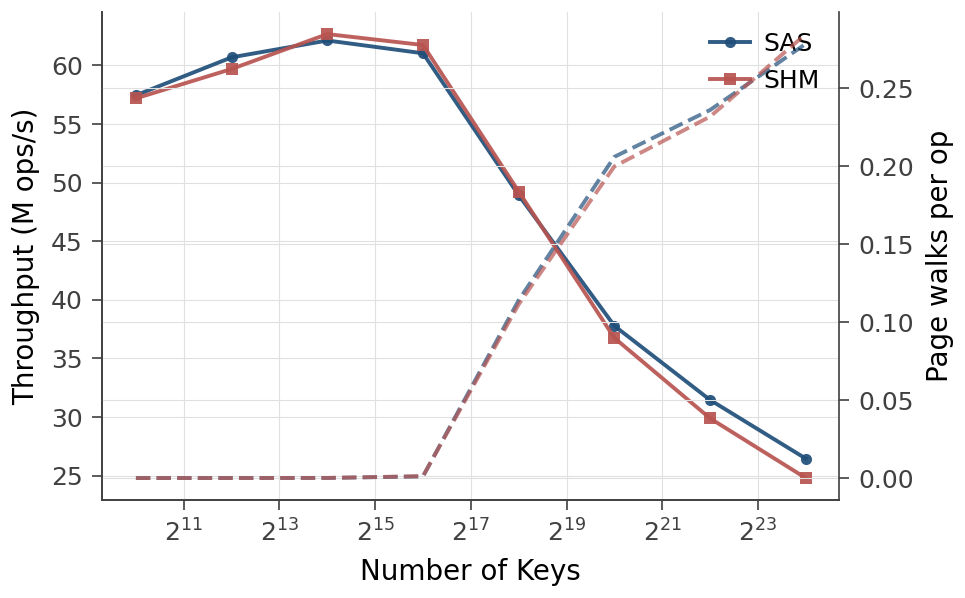
\includegraphics[width=\linewidth]{arch/num_keys/mixed_throughput.png}\\
            {\scriptsize\itshape Throughput + TLB misses vs. working set}
    \end{columns}
\end{frame}

\begin{frame}[standout]
	Questions?
\end{frame}

\end{document}
